\section{Interest rate dynamics for the risk-free asset}\label{sec:Interest_rate_dynamics}
In this section we try to extend the model presented in Chapter \ref{chpt:ED} by assuming a dynamics for the bank account interest rate. Starting from the portfolio dynamics (\ref{eq:ptf_dynamic_ED}), our aim is replacing it with
\begin{equation}\label{eq:portfolio_dynamic_Vasicek}
\boxed{x_{k+1} = x_k\Big( \exp\Big\{\int_{t_k}^{t_k+\tau_{k+1}}\!\!\!\!\!\!\!\!r_s\mathrm{d}s \Big\} + u_kJ\widetilde{N}_{k+1}\Big)} \qquad k \in \mathbb{N}
\end{equation}
where $\{r_t\}_{t\geq t_k}$ is the short-rate process and everything else remains unchanged from Chapter \ref{chpt:ED}. Due to its analytical tractability, we decided to model the short-rate according to the Vasicek Model (see \cite{brigo2007}). The following \gls{SDE} provides the dynamics of the short-rate
\begin{equation}\label{eq:VasicekSDE}
\begin{cases*}
dr_t = a(b-r_t)dt + \sigma dW_t\\
r_{t_k} = r_k, \qquad t \geq t_k
\end{cases*}
\end{equation}
where $a,b,\sigma$ and $r_k$ are positive constants and $\{W_t\}_{t\geq t_k}$ is a unidimensional Brownian motion. The main feature of the Vasicek model is the \textit{mean reversion} property: the process will tend to move to its average over time. Moreover, the process has a non-null probability of becoming negative. This is no longer a taboo since negative interest rates are observed in the market.

The solution of \gls{SDE} (\ref{eq:VasicekSDE}) is the following Ornstein–Uhlenbeck process
\begin{equation}\label{eq:solution_VasicekSDE}
r_t = r_ke^{-a(t-t_k)}+b(1-e^{-a(t-t_k)}) + \sigma e^{-a(t-t_k)}\int_{t_k}^{t}e^{a(s-t_k)}dW_s.
\end{equation}
However, we are interested in an explicit expression of the integral of process $r_t$ since it appears in the portfolio dynamics (\ref{eq:portfolio_dynamic_Vasicek}). Therefore, let us define the integrated short-rate process by $v_t=\int_{t_k}^{t}r_s\mathrm{d}s$. In order to find its explicit form, we integrate (\ref{eq:VasicekSDE}) from $t_k$ to a generic instant $t$, obtaining
\begin{equation}\label{eq:integrated_VasicekSDE}
r_t = r_k + a\big(b(t-t_k) - v_t\big) + \sigma(W_t-W_{t_k}).
\end{equation}
After equating (\ref{eq:integrated_VasicekSDE}) and (\ref{eq:solution_VasicekSDE}) and solving for $v_t$ we get
\begin{equation}\label{eq:v_t}
v_t = \frac{1}{a}\Big[(r_k-b)(1-e^{-a(t-t_k)})+ab(t-t_k)+\sigma\int_{t_k}^{t}(1-e^{-a(t-s)})dW_s\Big].
\end{equation}
From Appendix \ref{app:IntegratedOU} and (Proposition 7.1, \cite{baldi2017}) we have that
\begin{align}
\nonumber
v_t & \sim \mathcal{N}\Big(\eta(t-t_k),\zeta^2(t-t_k)\Big)\\[2ex]
\label{eq:Vasicek_mean}
\eta(t-t_k) & = \mathbb{E}[v_t]= \frac{1}{a}\Big[(r_k - b)\big(1-e^{-a(t-t_k)}\big)+ab(t-t_k)\Big]\\[2ex]
\label{eq:Vasicek_variance}
\zeta^2(t-t_k) & = \Var{v_t}= \frac{\sigma^2}{2a^3}\Big[2a(t-t_k) + 4e^{-a(t-t_k)}-e^{-2a(t-t_k)}-3\Big]
\end{align}
where $t \in \mathbb{R}^{+}$.
\begin{remark}
	The parameters $\eta(t-t_k)$ and $\zeta(t-t_k)$ depends only on the difference $t-t_k$, therefore the distribution of $v_t$ is stationary. This fact will be particularly useful in the following since the distribution of $v_{t_k+t}$ (which is the one we are interested in) depends only on $t$.
\end{remark}
\subsection{The density of $x_{k+1}$}
The last step is finding the probability density function of the random variable $x_{k+1}$. 
\begin{proposition}
	Let $x_{k+1}$ be the random variable (\ref{eq:portfolio_dynamic_Vasicek}). Then, its probability density function is
	\begin{align*}
	f_{x_{k+1}}(z) &=\frac{p}{(z-\xi)}\bigg\{ \int_{0}^{\infty}\varphi\Big(\frac{\log\big(\frac{z-\xi}{x}\big)-\eta(t)}{\zeta(t)}\Big)\Big(\frac{1}{\zeta(t)}\Big)f_{\tau_{k+1}}(t)\mathrm{d}t\bigg\}\mathbbm{1}_{[x+\xi,\infty)} \nonumber +\\
	& + \frac{(1-p)}{(z+\xi)}\bigg\{ \int_{0}^{\infty}\varphi\Big(\frac{\log\big(\frac{z+\xi}{x}\big)-\eta(t)}{\zeta(t)}\Big)\Big(\frac{1}{\zeta(t)}\Big)f_{\tau_{k+1}}(t)\mathrm{d}t\bigg\}\mathbbm{1}_{[x-\xi,\infty)}
	\end{align*}
	where $\xi=xJu_k$, $f_{\tau_{k+1}}= \big\{\lambda e^{-\lambda t}\big\}\mathbbm{1}_{[0,\infty)}$ is the density of random variable $\tau_{k+1}$, $\varphi$ is the density of a standard normal and $\eta(t),\zeta(t)$ are function (\ref{eq:Vasicek_mean}) and the square root of (\ref{eq:Vasicek_variance}) respectively, computed in $t+t_k$.
\end{proposition}
\begin{proof}
	Let us rewrite the portfolio dynamics in the following way
	\[
	x_{k+1}=x\exp\{v_{t_k+\tau_{k+1}}\} + xJu_k\widetilde{N}_{k+1}=Y+\xi\widetilde{N}_{k+1}.
	\]
	The first step of the proof is finding the cdf of Y:
	\begin{align*}
	F_Y(y) & = \mathbb{P}\big(x\exp\{v_{t_k+\tau_{k+1}}\}\leq y\big)\\
	& = \int_{0}^{\infty}\mathbb{P}\Big(v_{t_k+\tau_{k+1}}\leq \log(y/x)\big\lvert \tau_{k+1}=t\Big)f_{\tau_{k+1}}(t)\mathrm{d}t\\
	& = \int_{0}^{\infty}\mathbb{P}\Big(v_{t_k+t}\leq \log(y/x)\Big)f_{\tau_{k+1}}(t)\mathrm{d}t\\
	& = \Bigg\{\int_{0}^{\infty}\Phi\Big(\frac{\log(y/x)-\eta(t)}{\zeta(t)}\Big)f_{\tau_{k+1}}(t)\mathrm{d}t \Bigg\}\mathbbm{1}_{[x,\infty)}
	\end{align*}
	where we used the Law of Total Probability in the continuous case and the fact that $v_{t_k+t}$ is Gaussian with parameters $\eta(t)$ and $\zeta(t)$ (which are the functions (\ref{eq:Vasicek_mean}) and the square root of (\ref{eq:Vasicek_variance}) respectively, computed in $t+t_k$). $\Phi$ is the cdf of a standard normal.
	
	
Repeating the usual steps, we are able to find the cdf of $x_{k+1}$:
\begin{align*}
F_{x_{k+1}}(z) & = \mathbb{P}\big(Y+\xi\widetilde{N}_{k+1}\leq z\big) \\
& = F_Y(z-\xi)p+F_Y(z+\xi)(1-p)\\
& = p\bigg\{ \int_{0}^{\infty}\Phi\Big(\frac{\log\big(\frac{z-\xi}{x}\big)-\eta(t)}{\zeta(t)}\Big)f_{\tau_{k+1}}(t)\mathrm{d}t\bigg\}\mathbbm{1}_{[x+\xi,\infty)}+\\
& + (1-p)\bigg\{ \int_{0}^{\infty}\Phi\Big(\frac{\log\big(\frac{z+\xi}{x}\big)-\eta(t)}{\zeta(t)}\Big)f_{\tau_{k+1}}(t)\mathrm{d}t\bigg\}\mathbbm{1}_{[x-\xi,\infty)}.
\end{align*}
where $p$ is the probability that $\widetilde{N}_{k+1}$ is equal to 1. Finally, deriving with respect to $z$ under the integral sign gives us the result.
\end{proof}

\subsection{The calibration of the Vasicek model}
In this section we see how parameters $a$, $b$ and $\sigma$ of the Vasicek model can be calibrated to data using the linear regression method. We closely follow \cite{Bernal2016}.

The first step is to discretize Equation (\ref{eq:VasicekSDE}) in order to find a linear relation between the short-rate process $r_t$ at time instants $t$ and $t+\Delta t$:
\begin{align}\label{eq:Vasicek_discretized}
\nonumber
r_{t+\Delta t} & = r_t + a(b-r_t)\Delta t+\sigma\sqrt{\Delta t}Z \\
& = (1-a\Delta t)r_t+ab\Delta t+\sigma\sqrt{\Delta t}Z
\end{align}
where $Z \sim \mathcal{N}(0,1)$. From (\ref{eq:Vasicek_discretized}) is clear the linear relation between $r_{t+\Delta t}$ and $r_t$. Therefore, the above equation can be rewritten in a fashion suitable for the linear regression estimation as follows
\[
r_{t+\Delta t} = \alpha r_t + \beta + \varepsilon
\]
where 
\begin{equation*}
\begin{cases*}
\alpha = 1-a\Delta t\\
\beta = ab\Delta t
\end{cases*}
\end{equation*}
and $\varepsilon \sim \mathcal{N}(0,\sigma^2\Delta t)$ is the error term. Let us suppose to have a random sample $\{r_1,\ldots,r_n\}$, for example daily 3-month LIBOR quotes. The independent variable and the response are
\[ \bm{y} = \begin{bmatrix}
r_2\\
\vdots\\
r_n
\end{bmatrix} \qquad
\bm{x}= \begin{bmatrix}
r_1\\
\vdots\\
r_{n-1}
\end{bmatrix}.
\]
The linear relation between $\bm{y}$ and $\bm{x}$ is reported in Figure (\ref{fig:linear_regression}).

\begin{figure}
	\centering
	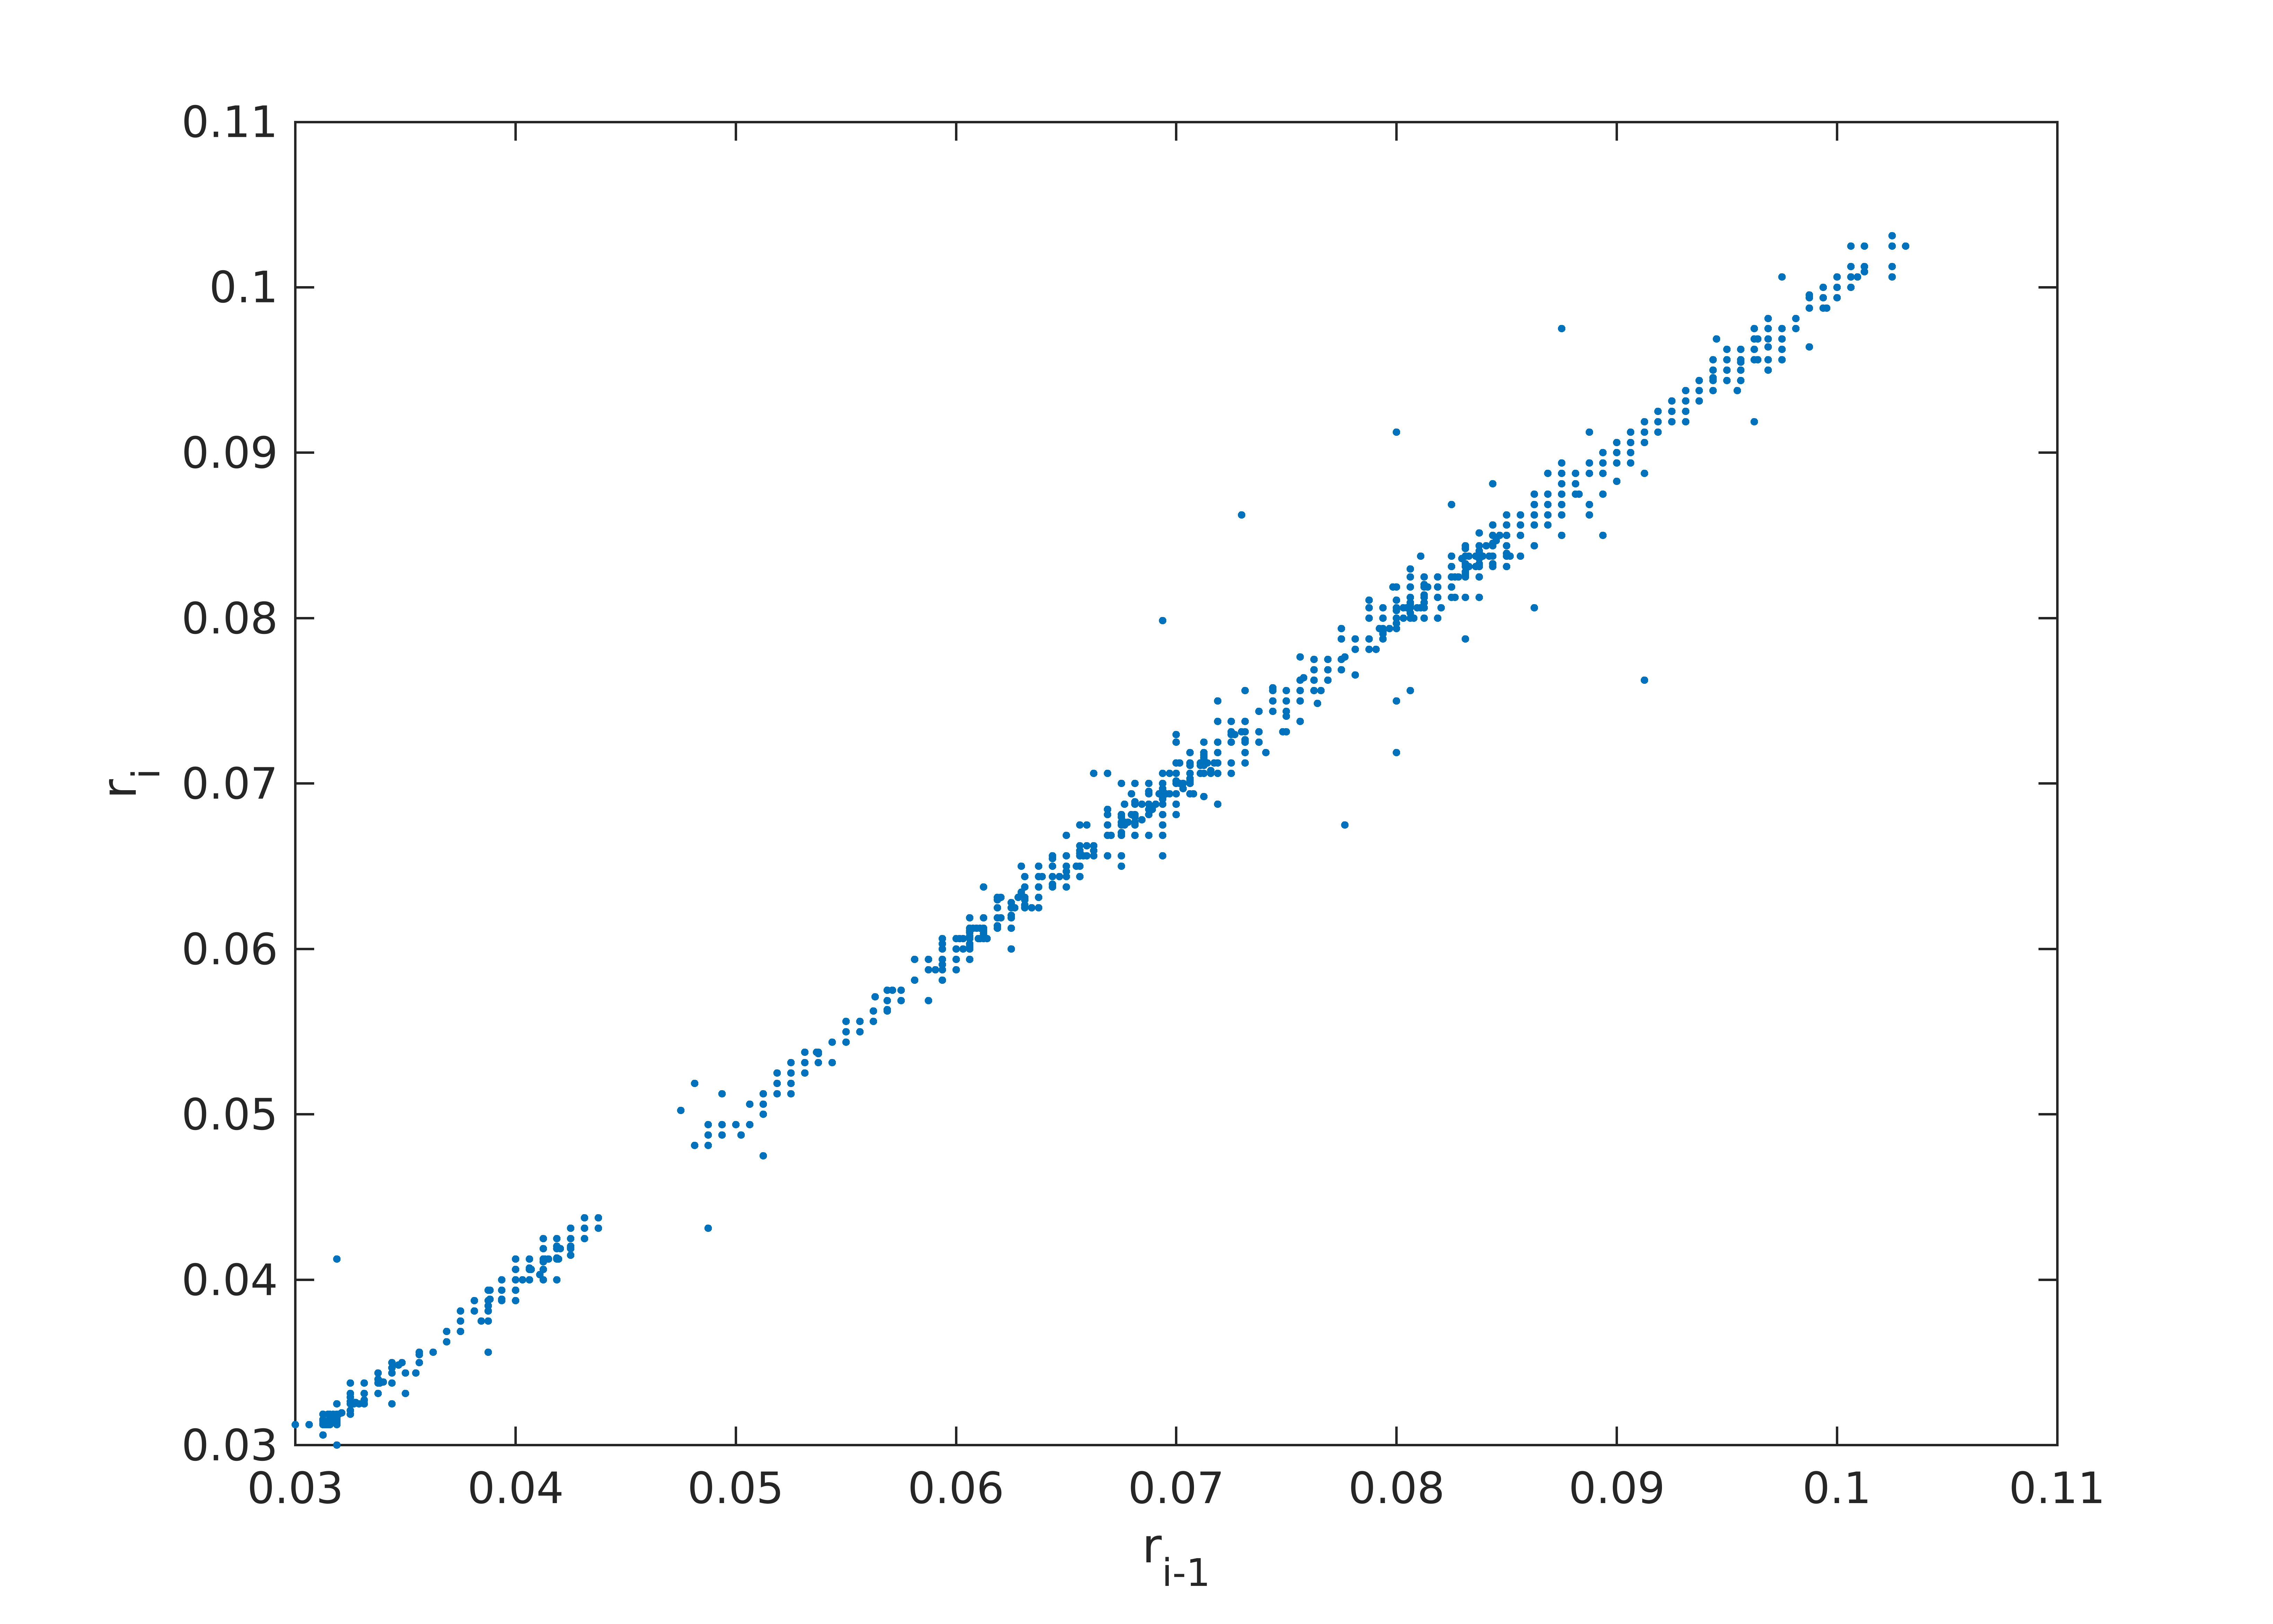
\includegraphics[scale=0.5]{Images/LinearRegression}
	\caption{Linear relation between consecutive daily 3-month LIBOR rate quotes. }
	\label{fig:linear_regression}
\end{figure}


Once the least square estimates $\widehat{\alpha}$ and $\widehat{\beta}$ have been found, we can recover the estimates of the Vasicek model parameters in the following way
\begin{equation*}
\begin{cases*}
\widehat{a}=\frac{1}{\Delta t}(1-\widehat{\alpha})\\[2ex]
\widehat{b}= \widehat{\beta}/(\widehat{a}\Delta t)\\[2ex]
\widehat{\sigma}=\frac{RSE}{\sqrt{\Delta t}}
\end{cases*}
\end{equation*}
where $RSE$ is the residual standard error of the fitting.

Applying this method to daily ($\Delta t = 1/252$) quotes of 3-month LIBOR starting from 22 January 2010 to 25 April 2016 brings the following estimates
\begin{equation*}
\begin{cases*}
\widehat{a}=0.1670\\
\widehat{b}=0.0280 \\
\widehat{\sigma}=0.0160.
\end{cases*}
\end{equation*}





